
    \documentclass{standalone}
\usepackage{tkz-fct}
\usepackage{tkz-euclide}
\usepackage{color}
\renewcommand*\familydefault{\sfdefault}
\usepackage{sansmath}
\sansmath
\definecolor{gray75}{gray}{0.75}
\begin{document}
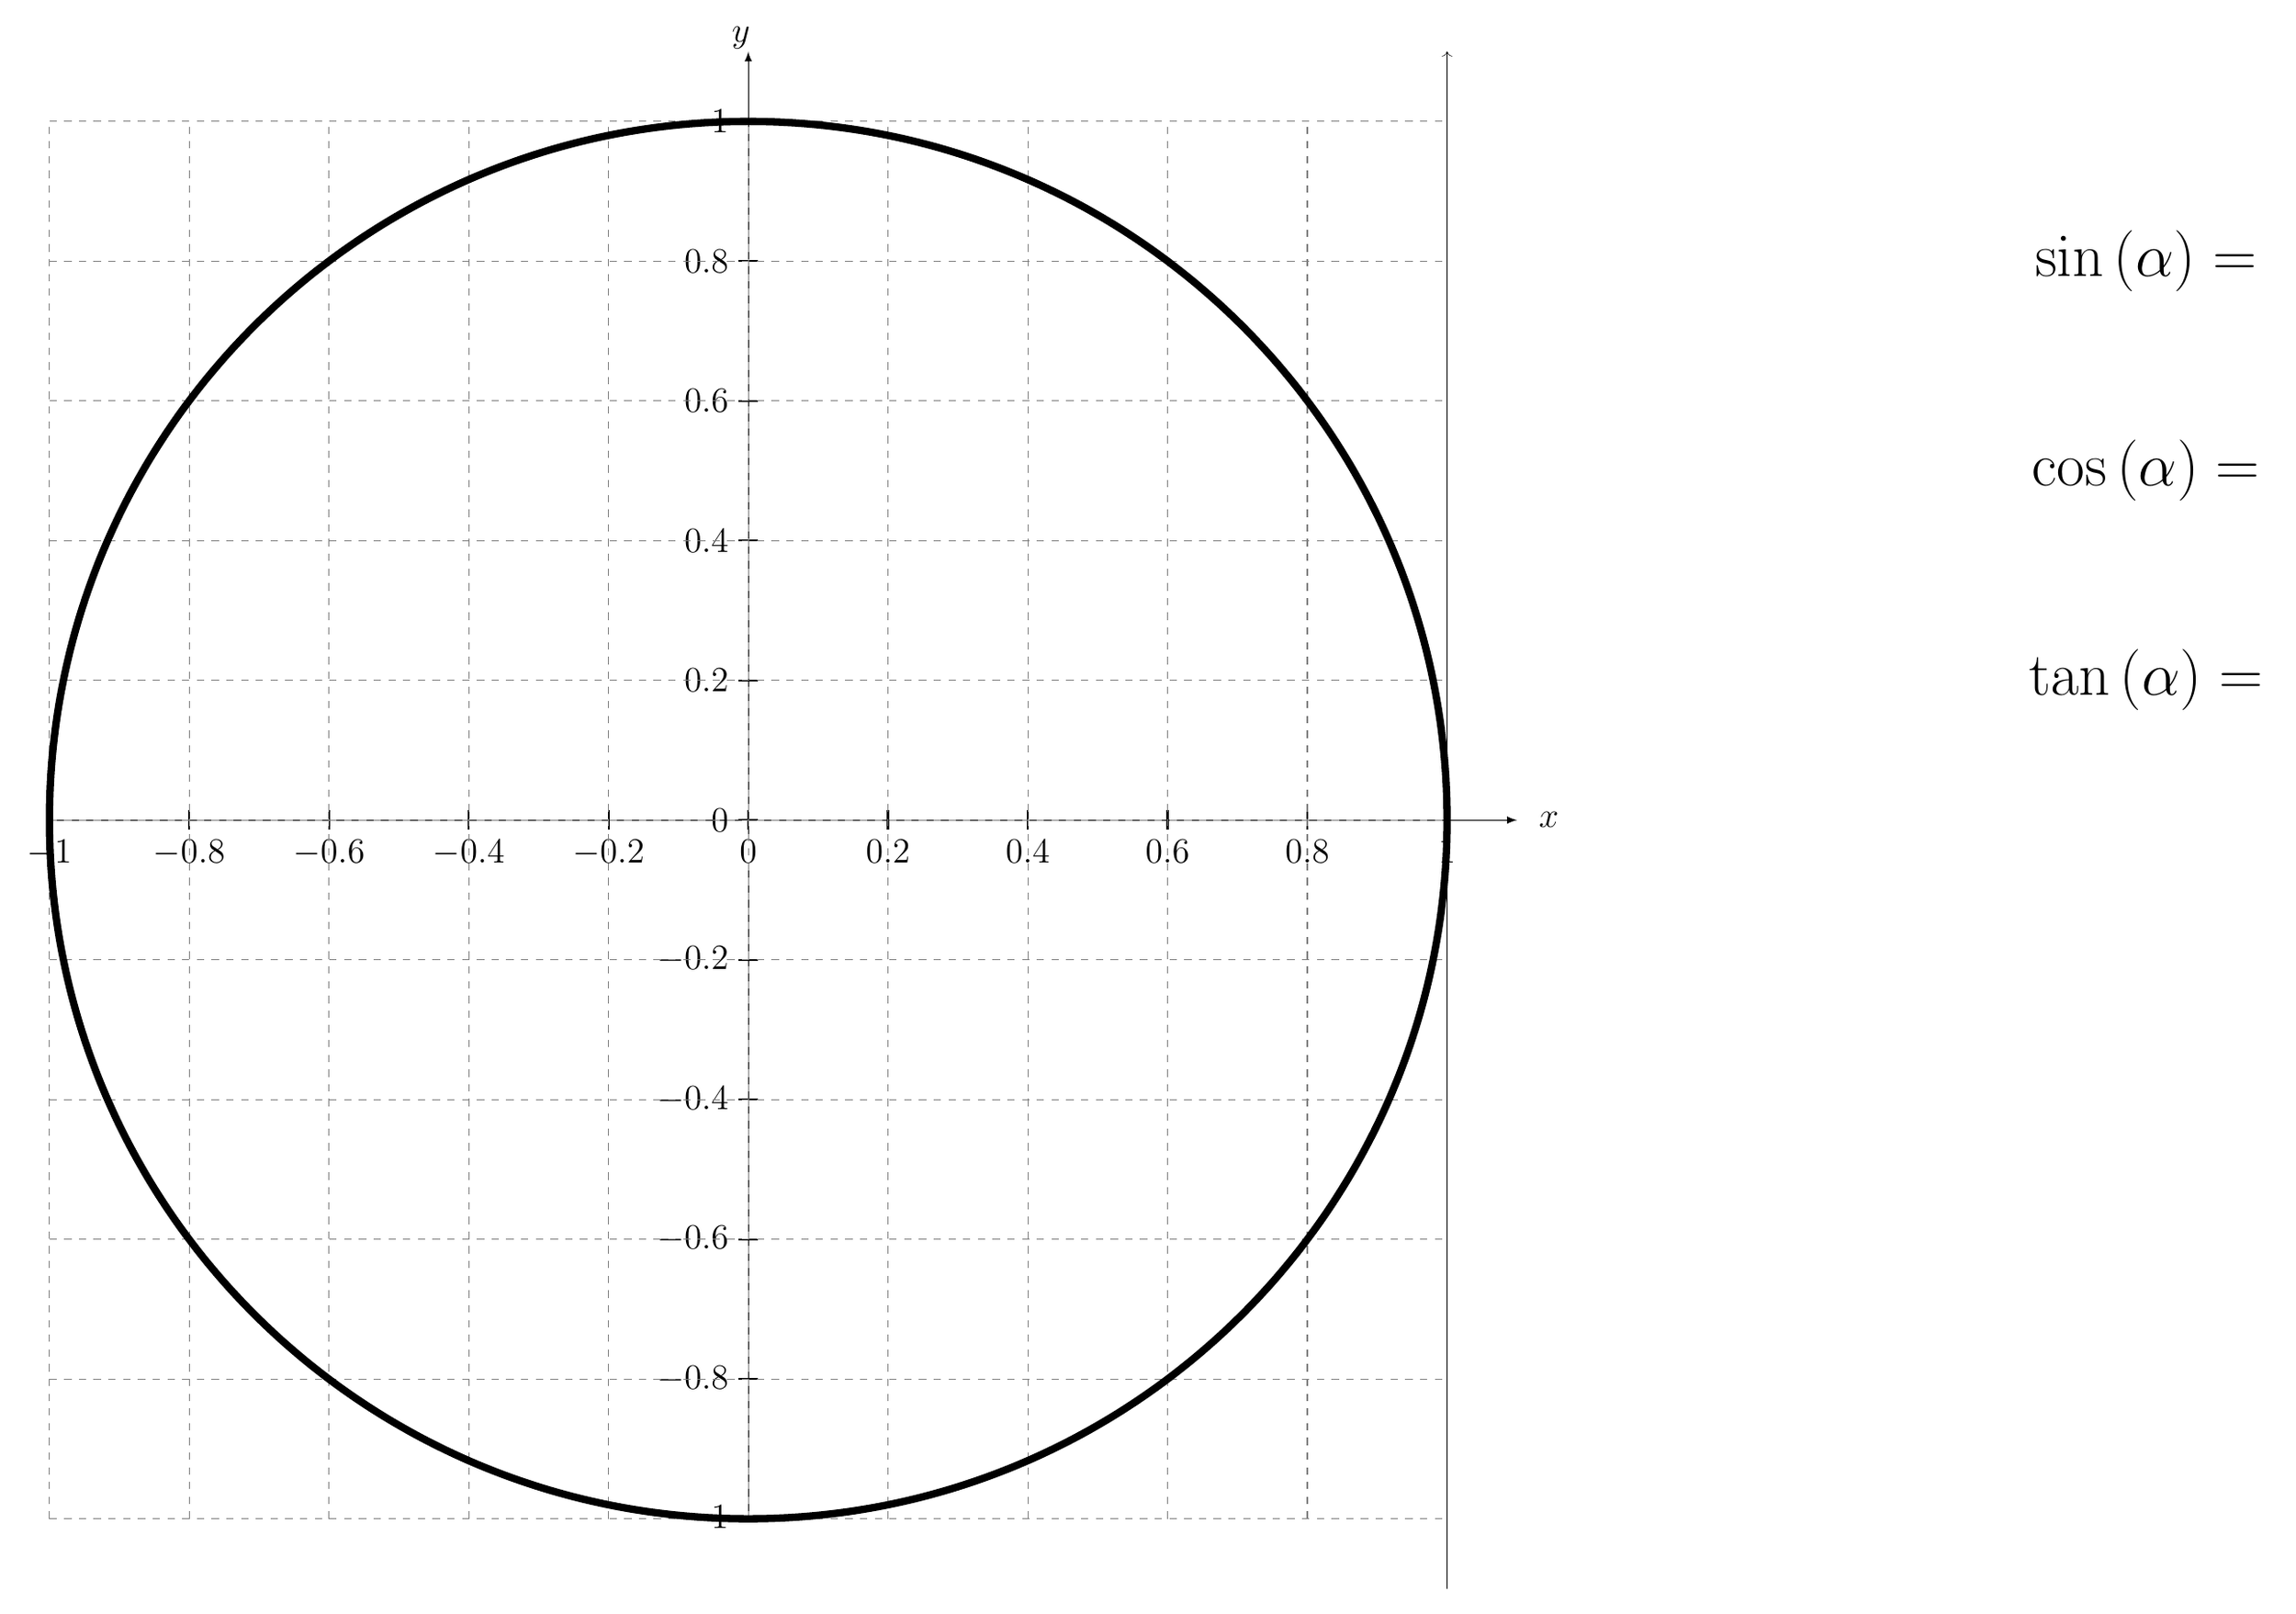
\begin{tikzpicture}[scale=2]
   \tkzInit[xmax=1.,ymax=1.,xmin=-1. ,ymin=-1,xstep=0.2,ystep=0.2]
   \tkzDrawY[ above, font=\Large]
   \tkzLabelY[node font=\Large]
   \tkzLabelX[node font=\Large]
   \tkzDrawX[right=8pt, font=\Large]
   \begin{scope}[dashed]
     \tkzGrid
   \end{scope}
   \tkzDefPoints{0/0/O,1/0/A}
   \tkzDrawCircle[line width=3pt, color=black](O,A)
   \tkzDefPoints{1/1.1/A,1/-1.1/B}
   \tkzDrawSegment[<-](A,B)
\tkzText(2,0.8){
  \Huge
  $\sin\left(\alpha\right)=$}
  \tkzText(2,0.5){\Huge$\cos\left(\alpha\right)=$}
  \tkzText(2,0.2){\Huge$\tan\left(\alpha\right)=$}
\end{tikzpicture}
\end{document}
